\documentclass[twocolumn]{article}
\usepackage{graphicx}
\usepackage[utf8]{inputenc}
\usepackage[a4paper, margin=0.79in]{geometry}
\usepackage{lastpage}
\usepackage[compact]{titlesec}

\titleformat{\section}[hang]{\bfseries\large}{\thesection}{0.5em}{}
\titleformat{\subsection}[hang]{\bfseries\normalsize}{\thesubsection}{0.5em}{}
\titleformat{\subsubsection}[runin]{\bfseries\normalsize}{\thesubsubsection}{0.5em}{}

\title{\large{\textbf{Systme Validation - Wafer Control}}}
\author{
    \small Ester Vicario ()
    \and \small Gerardo Moyers (4820800 , gmoyersbarrera)
    \and \small Teresa ()
      \and \small yuri ()
}
\date{}

\begin{document}

\maketitle

\begin{center}
    \footnotesize{Report contains \pageref{LastPage} of maximum 6 pages.}
\end{center}

\section{Introduction}
The System Validation course IN4387 is going to be dedicated to find the most efficient solution and validation of the production of silicon wafers. The goal of this assignment is to optimize and evaluate the preparation of the wafers using a control system. By evaluating the process in mcrl2 software it can be determined the feasibility of the implementation. 



\section{Requirements of the system}
During this part of the project and with the main objective of simplify the aspects of it, four components are gonna be considered: 1)the light, 2) both robots R1 and R2, 3) both air lockers with their respective output and input doors and 4) the robot R3.
The requirements of each component will be enumerate a continuation 


\begin{itemize}
\item Light requirements
\begin{itemize}
\item{The light should project the design  when there is a wafer in case there is no wafer it should remain switched off.}
\end{itemize}
\item Air lockers

\begin{itemize}
\item{Both output and input doors can not be open at the same time.}
\item{The  DOi doors should open when they detect that there is something at the input or that a wafer is ready to go to the output.}
\item{The input DIi doors should behave  opening when a wafer is ready to be designed in the lamp or is ready to be delivered to the output. }
\item{Doors should detect if there is any object that needs to enter in the air locker or leave it}

\end{itemize}
\item Robots R1 and R2
\begin{itemize}
\item {Robots must decide if taking an object of dropping in the input or output stacks depending on the airlockers availability an capacity of the stacks}
\item {Once noticed a wafer is  ready in the inputs robots should detect if the airlock is empty}
\item{A robot will have to check if the output stack is full before dropping a wafer}

\end{itemize}
\item Robot R3
\begin{itemize}
\item {Robot R3 will only move when the input doors are opening.}
\item {Robot R3 will not move to the light until the processing of the wafer has finished}
\end{itemize}
\end{itemize}


%Briefly describe the systems you have benchmarked on, and by which methods you have measured.

\section{Interactions and Architecture}
\subsection{Interactions}
The system has 4 elements that can have interactions; Robots R1, R2, Stack, Airlock, light and Robot R3.
\begin{itemize}
\item Robots R1, R2
\begin{itemize}
\item{pick a wafer}
\item{drop a wafer}
\item{go to input}
\item{go to output}
\item{go to airlock}
\item{request door open}
\item{ask for stack status}
\item{check door status}
\end{itemize}
\item Stack
\begin{itemize}
\item{ send status (Take me or Go away) }
\end{itemize}
\item Airlock
\begin{itemize}
\item{ open door}
\item{ close door}
\item{ check door status}
\item{ send door status}
\item{ airlock stuff (creates vacuum)}
\item{check if wafer present}
\item check if robot present
\end{itemize}
\item Robot R3
\begin{itemize}
\item{Pick/place wafer }
\item{Request door open}
\item{Check lamp status}
\item{ Check door status}
\end{itemize}
\end{itemize}
\begin{itemize}
 
\item Light
\begin{itemize}
 \item check if wafer present
\item lamp stuff (UV light on/off)
\item check for error
\item send status
\end{itemize}
\end{itemize}
\subsection{Architecture}
The lamp system is described in the picture \ref{fig:Lamp_architecture}
\begin{figure}[h]
    \centering
    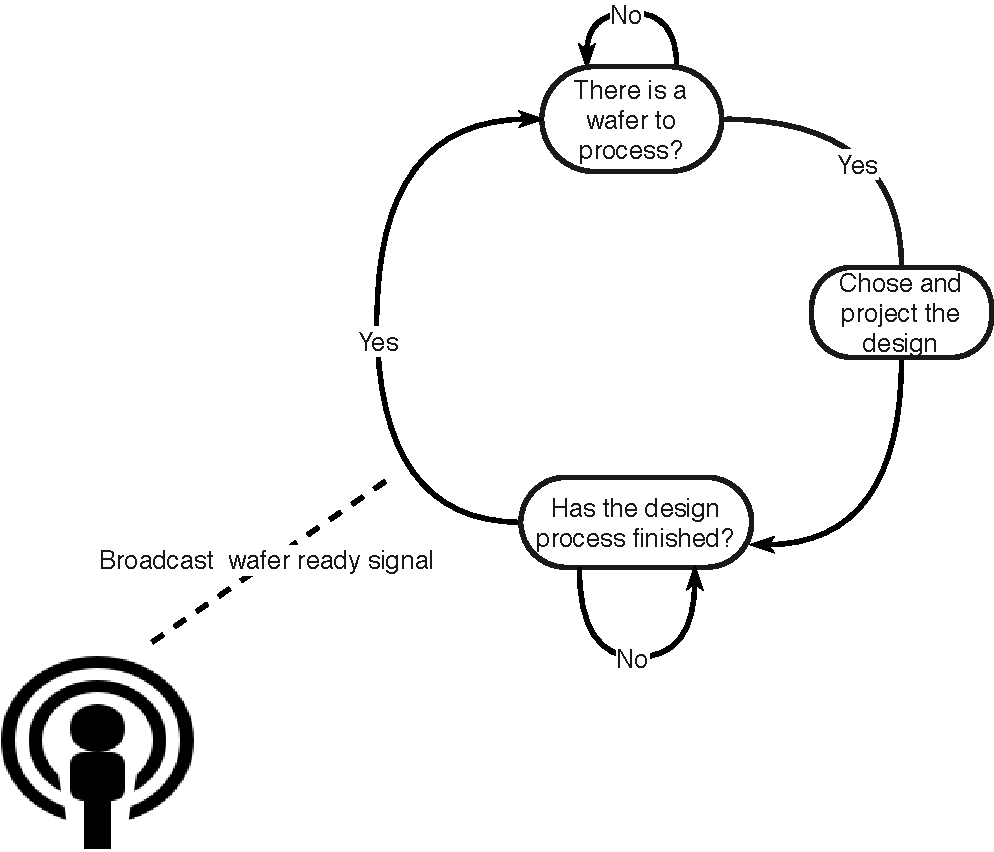
\includegraphics[width=0.45\textwidth]{lamp.pdf}
    \caption{Lamp architecture}
    \label{fig:Lamp_architecture}
\end{figure}
%Briefly describe and show graphs of the performance of your baseline implementation.
\subsection{Discussion}

%Briefly discuss / conclude peculiarities about this benchmark.

\section{Matrix multiplication}
\subsection{Description}
This benchmark tests the serial performance of a naive serial matrix multiplication that runs in $O(n^3)$ for square matrices with n columns. It will be used to compare the speed.
%Briefly describe this benchmark.

\subsection{Estimation}

%Briefly describe an estimation about the performance of matrix multiplication w.r.t. the vector baseline benchmark.
\subsection{Profile}
Briefly describe and show graphs of the performance of your baseline implementation.
\subsection{Discussion}
Briefly discuss / conclude peculiarities about this benchmark.

\section{SIMD extensions}
\subsection{Description}
SIMD is a type of computing technique focused on performing tasks in a quicker way. This benchmark uses vector operations so you can use 1 instruction to perform multiple operations.  
%Briefly describe this benchmark.
\subsection{Profile}
Briefly describe and show graphs of the performance of your baseline implementation.
\subsection{Estimation}
Briefly describe what improvements you can make based on the profile, and how much benefit it will give (in terms of e.g. speedup, throughput).
\subsection{Design and implementation}
Briefly describe all discrete improvements that you've made.
\subsubsection{Improvement X}
Your description goes here.
\subsubsection{Improvement Y}
\subsection{Results after improvement}
Briefly show the results after improvements.
\subsubsection{Results after improvement X}
\subsubsection{Results after improvement Y}
\subsection{Discussion}
Briefly discuss / conclude your work on this benchmark.

\section{OpenMP}
\subsection{Description}
Open Multi-Processing (OpenMP) is commonly. 
%Briefly describe this benchmark.
\subsection{Profile}
Briefly describe and show graphs of the performance of your baseline implementation.
\subsection{Estimation}
Briefly describe what improvements you can make based on the profile, and how much benefit it will give (in terms of e.g. speedup, throughput).
\subsection{Design and implementation}
Briefly describe all discrete improvements that you've made.
\subsubsection{Improvement X}
\subsubsection{Improvement Y}
\subsection{Results after improvement}
Briefly show the results after improvements.
\subsubsection{Results after improvement X}
\subsubsection{Results after improvement Y}
\subsection{Discussion}
Briefly discuss / conclude your work on this benchmark.

\section{OpenCL}
\subsection{Description}
Briefly describe this benchmark.
\subsection{Profile}
Briefly describe and show graphs of the performance of your baseline implementation.
\subsection{Estimation}
Briefly describe what improvements you can make based on the profile, and how much benefit it will give (in terms of e.g. speedup, throughput).
\subsection{Design and implementation}
Briefly describe all discrete improvements that you've made.
\subsubsection{Improvement X}
In the first version, compilation of the OpenCL program happened inside the matrix multiplication function. This compilation time took 0.3 seconds, giving lots of overhead. As an improvement, the code should be compiled once and the compiled program should be reused afterwards. Then, the only overhead is copying the Matrix from CPU memory to GPU memory.
\subsubsection{Improvement Y}
\subsection{Results after improvement}
Briefly show the results after improvements.
\subsubsection{Results after improvement X}
\subsubsection{Results after improvement Y}
\subsection{Discussion}
Briefly discuss / conclude your work on this benchmark.

\section{Conclusion}

\begin{thebibliography}{}
\bibitem{SomeReference} 
Some Author
\textit{Some Title}
Some Information about how to find this reference.
\end{thebibliography}

\end{document}
